%%%%%%%%%%%%%%%%%%%%%%%%%%%%%%%%%%%%%%%%%
% Lachaise Assignment
% LaTeX Template
% Version 1.0 (26/6/2018)
%
% This template originates from:
% http://www.LaTeXTemplates.com
%
% Authors:
% Marion Lachaise & François Févotte
% Vel (vel@LaTeXTemplates.com)
%
% License:
% CC BY-NC-SA 3.0 (http://creativecommons.org/licenses/by-nc-sa/3.0/)
%
%%%%%%%%%%%%%%%%%%%%%%%%%%%%%%%%%%%%%%%%%

%----------------------------------------------------------------------------------------
%	PACKAGES AND OTHER DOCUMENT CONFIGURATIONS
%----------------------------------------------------------------------------------------

\documentclass{article}

%%%%%%%%%%%%%%%%%%%%%%%%%%%%%%%%%%%%%%%%%
% Lachaise Assignment
% Structure Specification File
% Version 1.0 (26/6/2018)
%
% This template originates from:
% http://www.LaTeXTemplates.com
%
% Authors:
% Marion Lachaise & François Févotte
% Vel (vel@LaTeXTemplates.com)
%
% License:
% CC BY-NC-SA 3.0 (http://creativecommons.org/licenses/by-nc-sa/3.0/)
% 
%%%%%%%%%%%%%%%%%%%%%%%%%%%%%%%%%%%%%%%%%

%----------------------------------------------------------------------------------------
%	PACKAGES AND OTHER DOCUMENT CONFIGURATIONS
%----------------------------------------------------------------------------------------

\usepackage{amsmath,amsfonts,stmaryrd,amssymb} % Math packages

\usepackage{enumerate} % Custom item numbers for enumerations

\usepackage[ruled]{algorithm2e} % Algorithms

\usepackage[framemethod=tikz]{mdframed} % Allows defining custom boxed/framed environments

\usepackage{listings} % File listings, with syntax highlighting
\lstset{
	basicstyle=\ttfamily, % Typeset listings in monospace font
}
\usepackage{subcaption}

%----------------------------------------------------------------------------------------
%	DOCUMENT MARGINS
%----------------------------------------------------------------------------------------

\usepackage{geometry} % Required for adjusting page dimensions and margins

\geometry{
	paper=a4paper, % Paper size, change to letterpaper for US letter size
	top=2.5cm, % Top margin
	bottom=3cm, % Bottom margin
	left=2.5cm, % Left margin
	right=2.5cm, % Right margin
	headheight=14pt, % Header height
	footskip=1.5cm, % Space from the bottom margin to the baseline of the footer
	headsep=1.2cm, % Space from the top margin to the baseline of the header
	%showframe, % Uncomment to show how the type block is set on the page
}

%----------------------------------------------------------------------------------------
%	FONTS
%----------------------------------------------------------------------------------------

\usepackage[utf8]{inputenc} % Required for inputting international characters
\usepackage[T1]{fontenc} % Output font encoding for international characters

\usepackage{XCharter} % Use the XCharter fonts

%----------------------------------------------------------------------------------------
%	COMMAND LINE ENVIRONMENT
%----------------------------------------------------------------------------------------

% Usage:
% \begin{commandline}
%	\begin{verbatim}
%		$ ls
%		
%		Applications	Desktop	...
%	\end{verbatim}
% \end{commandline}

\mdfdefinestyle{commandline}{
	leftmargin=10pt,
	rightmargin=10pt,
	innerleftmargin=15pt,
	middlelinecolor=black!50!white,
	middlelinewidth=2pt,
	frametitlerule=false,
	backgroundcolor=black!5!white,
	frametitle={Command Line},
	frametitlefont={\normalfont\sffamily\color{white}\hspace{-1em}},
	frametitlebackgroundcolor=black!50!white,
	nobreak,
}

% Define a custom environment for command-line snapshots
\newenvironment{commandline}{
	\medskip
	\begin{mdframed}[style=commandline]
}{
	\end{mdframed}
	\medskip
}

%----------------------------------------------------------------------------------------
%	FILE CONTENTS ENVIRONMENT
%----------------------------------------------------------------------------------------

% Usage:
% \begin{file}[optional filename, defaults to "File"]
%	File contents, for example, with a listings environment
% \end{file}

\mdfdefinestyle{file}{
	innertopmargin=1.6\baselineskip,
	innerbottommargin=0.8\baselineskip,
	topline=false, bottomline=false,
	leftline=false, rightline=false,
	leftmargin=2cm,
	rightmargin=2cm,
	singleextra={%
		\draw[fill=black!10!white](P)++(0,-1.2em)rectangle(P-|O);
		\node[anchor=north west]
		at(P-|O){\ttfamily\mdfilename};
		%
		\def\l{3em}
		\draw(O-|P)++(-\l,0)--++(\l,\l)--(P)--(P-|O)--(O)--cycle;
		\draw(O-|P)++(-\l,0)--++(0,\l)--++(\l,0);
	},
	nobreak,
}

% Define a custom environment for file contents
\newenvironment{file}[1][File]{ % Set the default filename to "File"
	\medskip
	\newcommand{\mdfilename}{#1}
	\begin{mdframed}[style=file]
}{
	\end{mdframed}
	\medskip
}

%----------------------------------------------------------------------------------------
%	NUMBERED QUESTIONS ENVIRONMENT
%----------------------------------------------------------------------------------------

% Usage:
% \begin{question}[optional title]
%	Question contents
% \end{question}

\mdfdefinestyle{question}{
	innertopmargin=1.2\baselineskip,
	innerbottommargin=0.8\baselineskip,
	roundcorner=5pt,
	nobreak,
	singleextra={%
		\draw(P-|O)node[xshift=1em,anchor=west,fill=white,draw,rounded corners=5pt]{%
		Question \theQuestion\questionTitle};
	},
}

\newcounter{Question} % Stores the current question number that gets iterated with each new question

% Define a custom environment for numbered questions
\newenvironment{question}[1][\unskip]{
	\bigskip
	\stepcounter{Question}
	\newcommand{\questionTitle}{~#1}
	\begin{mdframed}[style=question]
}{
	\end{mdframed}
	\medskip
}

%----------------------------------------------------------------------------------------
%	WARNING TEXT ENVIRONMENT
%----------------------------------------------------------------------------------------

% Usage:
% \begin{warn}[optional title, defaults to "Warning:"]
%	Contents
% \end{warn}

\mdfdefinestyle{warning}{
	topline=false, bottomline=false,
	leftline=false, rightline=false,
	nobreak,
	singleextra={%
		\draw(P-|O)++(-0.5em,0)node(tmp1){};
		\draw(P-|O)++(0.5em,0)node(tmp2){};
		\fill[black,rotate around={45:(P-|O)}](tmp1)rectangle(tmp2);
		\node at(P-|O){\color{white}\scriptsize\bf !};
		\draw[very thick](P-|O)++(0,-1em)--(O);%--(O-|P);
	}
}

% Define a custom environment for warning text
\newenvironment{warn}[1][Warning:]{ % Set the default warning to "Warning:"
	\medskip
	\begin{mdframed}[style=warning]
		\noindent{\textbf{#1}}
}{
	\end{mdframed}
}

%----------------------------------------------------------------------------------------
%	INFORMATION ENVIRONMENT
%----------------------------------------------------------------------------------------

% Usage:
% \begin{info}[optional title, defaults to "Info:"]
% 	contents
% 	\end{info}

\mdfdefinestyle{info}{%
	topline=false, bottomline=false,
	leftline=false, rightline=false,
	nobreak,
	singleextra={%
		\fill[black](P-|O)circle[radius=0.4em];
		\node at(P-|O){\color{white}\scriptsize\bf i};
		\draw[very thick](P-|O)++(0,-0.8em)--(O);%--(O-|P);
	}
}

% Define a custom environment for information
\newenvironment{info}[1][Info:]{ % Set the default title to "Info:"
	\medskip
	\begin{mdframed}[style=info]
		\noindent{\textbf{#1}}
}{
	\end{mdframed}
}
 % Include the file specifying the document structure and custom commands
%Als we extra packages willen laden kan dat het best in structure.tex


% Define matices for pretty functions
\def\r{
	\begin{pmatrix}
		x \\
		y \\
		z 
	\end{pmatrix}}
	
\def\dr{
	\begin{pmatrix}
		\dot{x} \\
		\dot{y} \\
		\dot{z} 
	\end{pmatrix}}
	
\def\Nabla{
	\begin{pmatrix}
		\frac{\partial}{\partial {x}} \\
		\frac{\partial}{\partial {y}} \\
		\frac{\partial}{\partial {z}} 
	\end{pmatrix}}
	
\def\dNabla{
	\begin{pmatrix}
		\frac{\partial}{\partial \dot{x}} \\
		\frac{\partial}{\partial \dot{y}} \\
		\frac{\partial}{\partial \dot{z}} 
	\end{pmatrix}}
	
	
\begin{document}

\section{Principle of Fermat}

\textit{\underline{Question:} Proof that equation \ref{eq_1.3} and \ref{eq_1.4} can be reduced to equation \ref{eq_1.6}.} \\

\begin{equation}
	\label{eq_1.3}
	L[x,y,z,\dot{X},\dot{y},\dot{z}] = n(x,y,z)\sqrt{\dot{x}^2+\dot{y}^2+\dot{z}^2}
\end{equation}

\begin{equation}
	\label{eq_1.4}
	\frac{d}{dt} \frac{\partial L}{\partial \dot{x}} - \frac{\partial L}{\partial x} = 0, \frac{d}{dt} \frac{\partial L}{\partial \dot{y}} - \frac{\partial L}{\partial y} = 0, \frac{d}{dt} \frac{\partial L}{\partial \dot{z}} - \frac{\partial L}{\partial z} = 0
\end{equation}

\begin{equation}
	\label{eq_1.6}
	\frac{d}{ds} \left[ n \frac{d \vec{r}}{ds} \right] = \vec{\nabla} n
\end{equation} \\
\textit{\underline{Answer:}}\\
\\
First noting that $ds$ is a small element of distance travelled. Therefore taking into account the $x$, $y$ and $z$ direction, $ds$ is given by: \\

\begin{equation}
	ds = \sqrt{{dx}^2+{dy}^2+{dz}^2}
\end{equation}

A small distance travelled in a trivial direction, lets say $dx$, can be approximated by as $dx = dt \cdot \dot{x}$. Therefore $ds$ can be rewritten as: \\

\begin{equation}
	ds = dt \sqrt{\dot{x}^2+\dot{y}^2+\dot{z}^2}
\end{equation}

Rewriting gives:

\begin{equation}
	\label{eq_dsdt}
	\sqrt{\dot{x}^2+\dot{y}^2+\dot{z}^2} = \frac{ds}{dt}
\end{equation}

If we combine the equations in equation \ref{eq_1.4} in vector notation we get: \\

\begin{equation}
	\frac{d}{dt} \dNabla L - \nabla L = 0
\end{equation}

Rewriting and filling in equation \ref{eq_1.3} gives:

\begin{equation}
	\frac{d}{dt} \left[ \dNabla n(x,y,z)\sqrt{\dot{x}^2+\dot{y}^2+\dot{z}^2} \right] = \Nabla \left[ n(x,y,z)\sqrt{\dot{x}^2+\dot{y}^2+\dot{z}^2} \right]
\end{equation}

\begin{equation}
	\frac{d}{dt}  \frac{n \cdot \dot{\vec{r}} }{\sqrt{\dot{x}^2+\dot{y}^2+\dot{z}^2}}   = \vec{\nabla} n \; \sqrt{\dot{x}^2+\dot{y}^2+\dot{z}^2}
\end{equation}

Using equation \ref{eq_dsdt} to to replace the $\sqrt{\dot{x}^2+\dot{y}^2+\dot{z}^2}$ and rewriting the $\dot{\vec{r}}$ vector gives the following: \\

\begin{equation}
	\frac{d}{dt} \frac{n \cdot \dot{\vec{r}}}{\frac{ds}{dt}}  = \vec{\nabla} n \: \frac{ds}{dt}
\end{equation}

\begin{equation}
	\frac{d}{dt}  \frac{n \cdot \frac{d}{dt} \vec{r}}{\frac{ds}{dt}}   =  \vec{\nabla} n \: \frac{ds}{dt}
\end{equation}

Rewriting yields the equation that was to be proved: \\

\begin{equation}
	\frac{d}{ds} \left[ n \frac{d \vec{r}}{ds} \right] = \vec{\nabla} n
\end{equation}

\section{Application}
\subsection{Homogeneous medium}

\textit{\underline{Question:} Using equation \ref{eq_1.6}, show how light is travelling in a homogeneous medium.}\\
\\
\textit{\underline{Answer:}} \\
\\
Equation \ref{eq_1.6} can be rewritten using the chain rule: \\

\begin{equation}
	\frac{d \vec{r}}{ds} \frac{d}{ds} n + n \frac{d^2 \vec{r}}{ds^2} = \Nabla n
\end{equation} \\

Note that for a homogeneous medium, the index of refraction, $n$, is constant. Therefore $\frac{dn}{ds} = 0$, $\frac{\partial n}{\partial x} = 0$, $\frac{\partial n}{\partial y} = 0$ and $\frac{\partial n}{\partial z} = 0$. Using this in the previous equation yields: \\

\begin{equation}
	 n \frac{d^2 \vec{r}}{ds^2} = \vec{0}
\end{equation}

\begin{equation}
	 \frac{d^2 \vec{r}}{ds^2} = \vec{0}
\end{equation} \\


This implies that the direction and velocity of the light is not changed as the light travels through the medium. Therefore, it travels in a straight line with a constant velocity of $ v = c/n $. \\

\subsection{Snell-Descartes Law}

\textit{\underline{Question:} Express first geometrically and then analytically Snell and Descartes law of reflection and transmission of the light at the interface between two media of different index of refraction $n_1$ and $n_2$, using the Principle of Fermat and equation \ref{eq_1.6}.}\\
\\
\textit{\underline{Answer:}} \\
\\

\subsubsection{Geometrical}
The speed of light in a medium is inversely proportional to the refractive index. Therefore, the shortest path (in distance) between two points in materials with different refractive indices is not always the fastest (in time). This phenomenon is nicely described by a 2-dimensional analogy of a beach (see figure \ref{fig_snell_empty}). The maximum speed on foot on beach is significantly higher than the maximum swimming speed in the water. So if somebody would need to get from a point A on the beach to a point B in the water, the direct route from A to B (dashed line in figure \ref{fig_snell_empty}) would intuitively be slower than the path with a shorter swimming distance (solid line in figure \ref{fig_snell_empty}). 

\begin{figure}[h!]
	\centering
	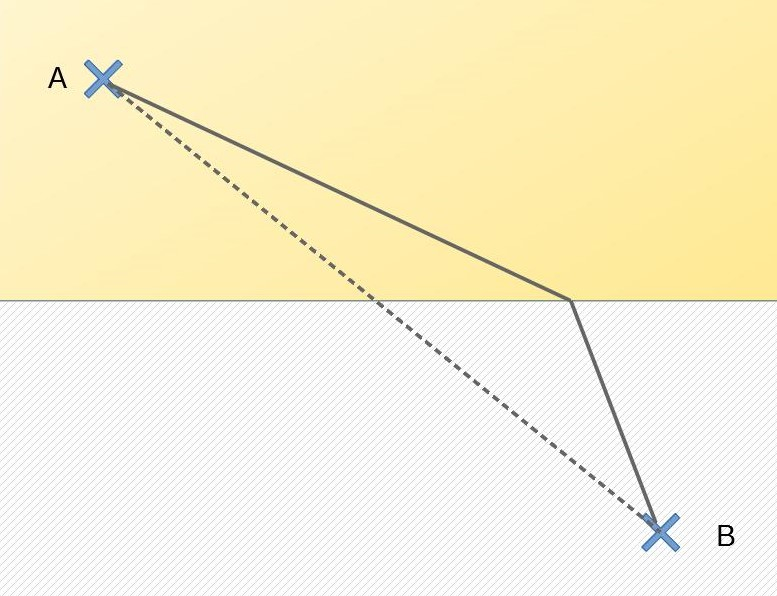
\includegraphics[width=8cm]{afbeeldingen/snell_diagram_leeg.jpg}
	\caption{Diagram of a 2-dimensional beach analogy of the interface between two media with different index of refraction. The upper-half corresponds to the beach and the lower-half to the sea. The dashed line corresponds to the direct route between point A and B with the shortest distance. The solid line corresponds to a route that is intuitively faster than the direct route.}
	\label{fig_snell_empty}
\end{figure}

It is possible to calculate the fastest route between point A and B If we add the parameters $v_1$, $v_2$, $\theta _1$, $\theta _2$, $a$, $b$, $c$ and $d$ which corresponds respectively to the propagation speed on the beach, the propagation speed in the water, the angle of the path on the beach with the normal, the angle of the path in the water with the normal and distances which can be seen in figure \ref{fig_snell_full}. 

\begin{figure}[h!]
	\centering
	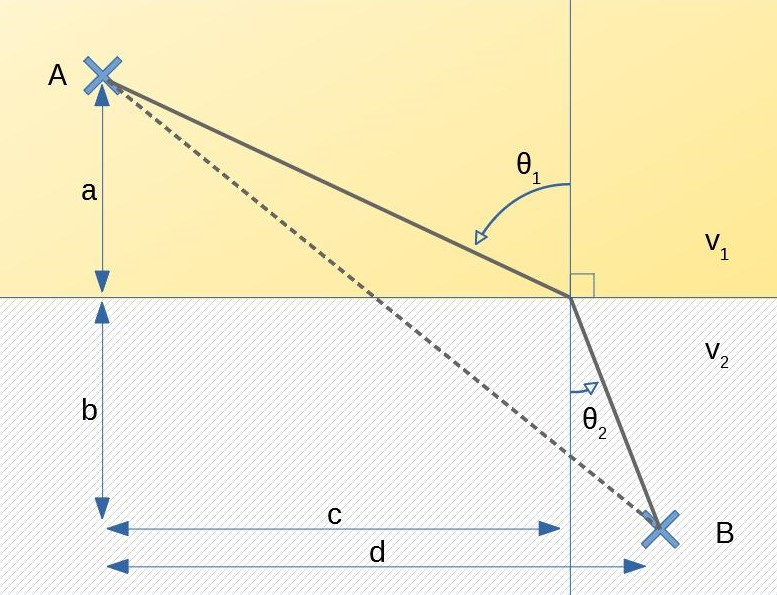
\includegraphics[width=8cm]{afbeeldingen/snell_diagram_vol.jpg}
	\caption{Diagram of beach analogy parameters $v_1$, $v_2$, $\theta _1$, $\theta _2$, $a$, $b$, $c$ and $d$. These correspond respectively to the propagation speed on the beach, the propagation speed in the water, the angle of the path on the beach with the normal, the angle of the path in the water with the normal and distances which can be seen in the diagram.}
	\label{fig_snell_full}
\end{figure} 

The time it takes to travel from point A to B, $t$, can easily be found dividing the path on the beach and the water, respectively $l_{beach}$ and $l_{water}$ by the corresponding speed: 

\begin{equation}
	t = l_{beach}/v_1 + l_{water}/v_2
\end{equation} 

Using the pythagoras theorem we find: 

\begin{equation}
	t = \sqrt{a^2 + c^2}/v_1 + \sqrt{b^2 + (d-c)^2}/v_2
	\label{eq_t}
\end{equation} 

If there is a fastest path, there should be an optimum value for $c$ for which $dt/dc = 0$. Therefore, applying the principle of Fermat to equation \ref{eq_t} leads to the following: 

\begin{equation}
	0 = \frac{c}{v_1 \sqrt{a^2 + c^2}} + \frac{c-d}{v_2 \sqrt{b^2 + (d-c)^2}}
\end{equation}

Using the trigonometric identity $sin(\theta) = (adjacent side)/(diagonal side)$ for right-angled triangle we obtain: 

\begin{equation}
	0 =  sin(\theta _1)/v_1 - sin(\theta _2)/v_2
\end{equation}

If we rewrite this and use the fact that the speed of light in a medium is given by $v = c/n$ we obtain Snell-Descartes law: 

\begin{equation}
	n_1 \; sin(\theta _1) = n_2 \; sin(\theta _2) 
\end{equation}

This equation basically tells us, that for a interface to a higher refractive index, so where the light slows down, the light bends to the normal. 

\subsubsection{Analytical}

For the analytical derivation of Snell-Descartes law we will use a similar diagram as in the geometrical derivation with a coordinate system added as in figure \ref{fig_snell_analytical}.

\begin{figure}[h!]
\centering
  \begin{subfigure}[b]{0.6\textwidth}
    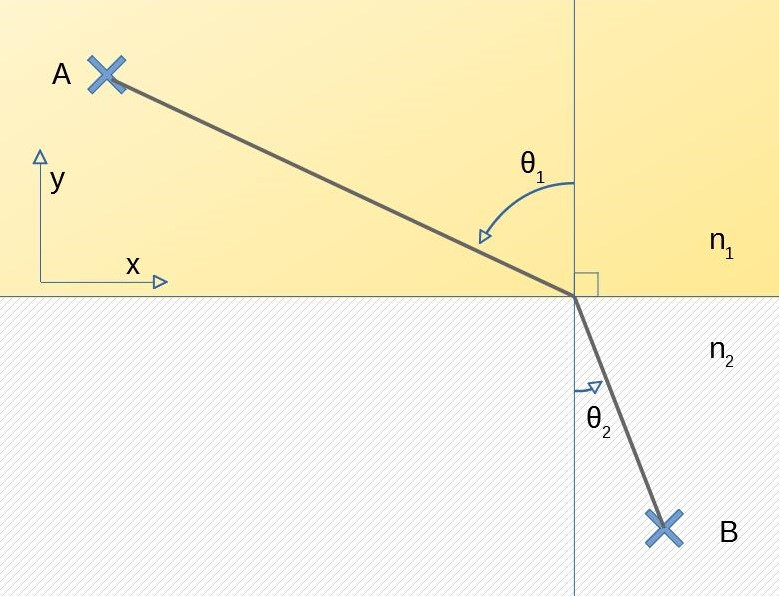
\includegraphics[width=\textwidth]{afbeeldingen/snell_analytical.jpg}
	\caption{Diagram of the path of light at the interface of two media with different refractive indices $n_1$ and $n_2$. $\theta _1$ and $\theta _2$ correspond to the angle with the normal.}
	\label{fig_snell_analytical}
  \end{subfigure}
  %
  \begin{subfigure}[b]{0.2\textwidth}
    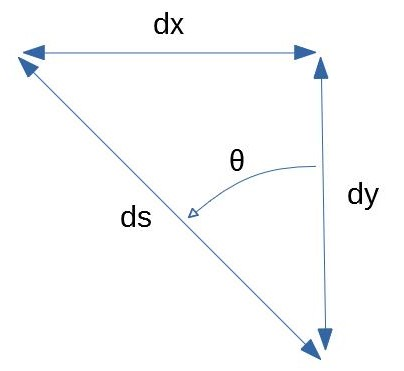
\includegraphics[width=\textwidth]{afbeeldingen/ds.jpg}
	\caption{$ds$ in relation to $dx$ and $dy$.}
	\label{fig_ds}
  \end{subfigure}
  \caption{}
\end{figure}


If we write equation \ref{eq_1.6} for only the x-component and use the fact that $n$ is independent of $x$ in our diagram, we get the following:

\begin{equation}
	\frac{d}{ds} \left[ n \frac{d x}{ds} \right] = \frac{d n}{dx}
\end{equation}

\begin{equation}
	\frac{d}{ds} \left[ n \frac{d x}{ds} \right] = 0
\end{equation}

The $ds$ in the latter equation is defined as in figure \ref{fig_ds}. If we keep a fixed $ds$ for both media we obtain the following equality:

\begin{equation}
	\frac{d}{ds} \left[ n_1 \frac{d x_1}{ds} \right] = \frac{d}{ds} \left[ n_2 \frac{d x_2}{ds} \right]
\end{equation}

Rewriting and using the trigonometric identity, $sin(\theta)= dx/ds$, yields the Snell-Descartes law:

\begin{equation}
	n_1 \frac{d x_1}{ds}]=n_2 \frac{d x_2}{ds}
\end{equation}

\begin{equation}
	n_1 \; sin(\theta _1) = n_2 \; sin(\theta _2)
\end{equation}





\end{document}
